\documentclass[12pt,a4paper]{report}
\usepackage[utf8]{inputenc}
\usepackage[T1]{fontenc}
\usepackage{mathptmx}
\usepackage{microtype}
\usepackage{geometry}
\geometry{a4paper, left=1.25in, right=1in, top=1in, bottom=1in}
\usepackage{graphicx}
\usepackage{amsmath,amssymb,amsfonts}
\usepackage{booktabs}
\usepackage{longtable}
\usepackage{array}
\usepackage{multirow}
\usepackage{xcolor}
\usepackage{setspace}
\usepackage{fancyhdr}
\usepackage{listings}
\usepackage{tikz}
\usetikzlibrary{arrows.meta,positioning,shapes.geometric,fit,calc,backgrounds}
\usepackage{pgfplots}
\pgfplotsset{compat=1.18}
\usepackage[font=small,labelfont=bf,labelsep=period]{caption}
\usepackage{titlesec}
\usepackage[nottoc]{tocbibind}
\usepackage[colorlinks=true, linkcolor=blue!50!black, citecolor=blue!50!black,
            urlcolor=blue!50!black, bookmarksnumbered=true]{hyperref}

\definecolor{pgnavy}{HTML}{1B365D}
\definecolor{pgteal}{HTML}{007A78}
\definecolor{pgamber}{HTML}{C66E00}
\definecolor{pgcrimson}{HTML}{B02A37}
\definecolor{pgslate}{HTML}{F2F5F8}
\definecolor{pgborder}{HTML}{8FA3B8}
\definecolor{pcumaroon}{HTML}{8B1D24}
\definecolor{pcudark}{HTML}{231F20}

% Official PCU Logo helper: uses logo.png / pcu_logo.png / logo.jpg when present,
% with a vector TikZ PCU crest + lockup fallback if compiled before uploading logo.png
\newcommand{\PCULogoVector}{%

\begin{tikzpicture}[x=1cm,y=1cm,baseline=(current bounding box.center)]
  \draw[line width=1.5pt, draw=pcudark, fill=white]
    (0,2.55) -- (1.82,2.55) -- (1.82,1.25)
    .. controls (1.82,0.52) and (1.32,0.12) .. (0.91,-0.12)
    .. controls (0.50,0.12) and (0,0.52) .. (0,1.25) -- cycle;
  \node[font=\fontsize{6}{6}\selectfont, text=pcumaroon] at (0.28,2.22) {$\star\star$};
  \node[font=\fontsize{12.5}{12.5}\selectfont\bfseries, text=pcudark] at (0.91,2.22) {PCU};
  \node[font=\fontsize{6}{6}\selectfont, text=pcumaroon] at (1.54,2.22) {$\star\star$};
  \fill[pcumaroon] (0.91,1.62) circle (0.145);
  \fill[pcumaroon]
    (0.89,0.10) -- (0.76,0.58)
    .. controls (0.35,0.78) and (0.16,1.22) .. (0.18,1.86)
    .. controls (0.40,1.62) and (0.64,1.38) .. (0.81,0.96)
    -- (0.89,0.96) -- cycle;
  \draw[white, line width=0.9pt] (0.18,1.52) .. controls (0.42,1.36) and (0.60,1.20) .. (0.76,1.02);
  \draw[white, line width=0.9pt] (0.22,1.20) .. controls (0.44,1.08) and (0.60,0.96) .. (0.76,0.82);
  \fill[pcumaroon]
    (0.93,0.10) -- (1.06,0.58)
    .. controls (1.47,0.78) and (1.66,1.22) .. (1.64,1.86)
    .. controls (1.42,1.62) and (1.18,1.38) .. (1.01,0.96)
    -- (0.93,0.96) -- cycle;
  \draw[white, line width=0.9pt] (1.64,1.52) .. controls (1.40,1.36) and (1.22,1.20) .. (1.06,1.02);
  \draw[white, line width=0.9pt] (1.60,1.20) .. controls (1.38,1.08) and (1.22,0.96) .. (1.06,0.82);
  \fill[white] (0.82,0.90) -- (1.00,0.90) -- (0.91,0.44) -- cycle;
  \fill[pcumaroon] (0.91,0.70) circle (0.045);
  \draw[pcumaroon, line width=0.8pt] (0.91,0.70) -- (0.91,0.16);
  \draw[line width=1.4pt, draw=pcudark] (2.22,-0.12) -- (2.22,2.58);
  \node[anchor=west, font=\fontsize{12}{13}\selectfont\bfseries, text=pcudark] at (2.48,2.35) {PCET's};
  \node[anchor=west, font=\fontsize{17}{18}\selectfont\bfseries, text=pcudark] at (2.48,1.72) {Pimpri};
  \node[anchor=west, font=\fontsize{17}{18}\selectfont\bfseries, text=pcudark] at (2.48,1.02) {Chinchwad};
  \node[anchor=west, font=\fontsize{17}{18}\selectfont\bfseries, text=pcudark] at (2.48,0.30) {University, Pune};
  \node[font=\fontsize{9.5}{11}\selectfont\sffamily, text=pcudark] at (3.25,-0.52)
    {Learn \textcolor{pcumaroon}{\textbf{|}} Grow \textcolor{pcumaroon}{\textbf{|}} Achieve};
\end{tikzpicture}%
}
\newcommand{\PCULogo}[1]{%
  \IfFileExists{logo.png}{
\includegraphics[height=#1]{logo.png}}{%
    \IfFileExists{pcu_logo.png}{\includegraphics[height=#1]{pcu_logo.png}}{%
      \IfFileExists{logo.jpg}{\includegraphics[height=#1]{logo.jpg}}{%
        \resizebox{!}{#1}{\PCULogoVector}%
      }%
    }%
  }%
}

\onehalfspacing
\setlength{\parindent}{0pt}
\setlength{\parskip}{6pt}
\setlength{\headheight}{15pt}
\emergencystretch=1.6em

% Prevent Overfull \hbox warnings in Table of Contents / List of Figures / Tables
\makeatletter
\renewcommand{\@pnumwidth}{2.65em}
\renewcommand{\@tocrmarg}{3.55em}
\makeatother

% Chapter and section heading formatting
\titleformat{\chapter}[display]
  {\normalfont\bfseries}{\centering\Large \MakeUppercase{\chaptertitlename}\ \thechapter}{10pt}{\centering\huge}
\titleformat{name=\chapter,numberless}[block]
  {\normalfont\huge\bfseries\centering}{}{0pt}{}
\titlespacing*{\chapter}{0pt}{-6pt}{20pt}
\titleformat{\section}{\normalfont\Large\bfseries}{\thesection}{0.8em}{}
\titleformat{\subsection}{\normalfont\large\bfseries}{\thesubsection}{0.8em}{}

% ---- Editable Metadata Macros -------------------------------------------
\newcommand{\AcademicYear}{2025--2026}
\newcommand{\ProjectTitle}{PhishGuard-Stack: Deception-Aware Multi-View URL Feature Engineering and Calibrated Dual-Modal Stacking for Fetch-Free Phishing Detection}
\newcommand{\ShortTitle}{PhishGuard-Stack: Fetch-Free Phishing Detection}
% -------------------------------------------------------------------------

\lstset{
  basicstyle=\ttfamily\footnotesize,
  breaklines=true,
  frame=single,
  columns=fullflexible,
  keepspaces=true
}

\tikzset{
  box/.style={draw=pgnavy, rounded corners=2.5pt, minimum height=9mm, minimum width=26mm,
              align=center, font=\small, fill=pgnavy!6, line width=0.55pt},
  boxg/.style={box, draw=pgteal, fill=pgteal!10},
  boxo/.style={box, draw=pgamber!85!black, fill=pgamber!12},
  boxr/.style={box, draw=pgcrimson, fill=pgcrimson!10},
  dec/.style={draw=pgnavy, diamond, aspect=2.3, align=center, font=\footnotesize,
              fill=yellow!14, inner sep=1.5pt, line width=0.55pt},
  arr/.style={-{Latex[length=2.2mm]}, thick, draw=pgnavy},
  lab/.style={font=\scriptsize, midway}
}

% Running headers and footers
\pagestyle{fancy}
\fancyhf{}
\lhead{\small\textit{Technical Seminar Report}}
\rhead{\small\textit{\ShortTitle}}
\lfoot{\small Dept.\ of Computer Science \& Engineering, PCU Pune}
\rfoot{\small Page \thepage}
\renewcommand{\headrulewidth}{0.4pt}
\renewcommand{\footrulewidth}{0.4pt}
\fancypagestyle{plain}{%
  \fancyhf{}
  \lfoot{\small Dept.\ of Computer Science \& Engineering, PCU Pune}
  \rfoot{\small Page \thepage}
  \renewcommand{\headrulewidth}{0pt}
  \renewcommand{\footrulewidth}{0.4pt}}

\begin{document}

% =========================== TITLE PAGE =================================
\hypersetup{pageanchor=false}
\begin{titlepage}
\singlespacing
\setlength{\parskip}{0pt}
\begin{tikzpicture}[remember picture, overlay]
  \draw[line width=1.8pt, draw=pgnavy] ($(current page.north west)+(0.68in,-0.68in)$) rectangle ($(current page.south east)+(-0.68in,0.68in)$);
  \draw[line width=0.6pt, draw=pgnavy] ($(current page.north west)+(0.75in,-0.75in)$) rectangle ($(current page.south east)+(-0.75in,0.75in)$);
\end{tikzpicture}
\centering
\vspace*{0.06in}
\PCULogo{1.08in}\\[0.12in]
{\large \textbf{SCHOOL OF ENGINEERING \& TECHNOLOGY}}\\[3pt]
{\normalsize \textbf{Department of Computer Science \& Engineering}}\\[0.20in]
{\large \textbf{A TECHNICAL SEMINAR REPORT ON}}\\[0.12in]
{\Large \textbf{\ProjectTitle}}\\[0.18in]
\textit{Submitted in partial fulfilment of the requirements for the degree of}\\[0.08in]
{\large \textbf{Bachelor of Technology}}\\[0.04in]
\textit{in}\\[0.04in]
{\large \textbf{Computer Science \& Engineering}}\\[0.20in]
\textbf{Submitted by:}\\[0.08in]
\begin{tabular}{ll}
\textbf{Kedar Kapse}    & \texttt{kedar.kapse24@pcu.edu.in} \\
\textbf{Ritesh Kumar}   & \texttt{ritesh.kumar24@pcu.edu.in} \\
\textbf{Saksham Sharma} & \texttt{saksham.sharma24@pcu.edu.in} \\
\textbf{Saurabh Singh}  & \texttt{saurabh.singh24@pcu.edu.in} \\
\end{tabular}\\[0.20in]
\textbf{Under the Guidance of:}\\[0.06in]
{\large \textbf{Dr.\ Avinash Golande}}\\[0.03in]
\textit{Professor, Department of Computer Science \& Engineering}
\vfill
\textbf{Department of Computer Science \& Engineering}\\
\textbf{School of Engineering \& Technology}\\
\textbf{Pimpri Chinchwad University, Pune, Maharashtra -- 412106, India}\\
\textbf{Academic Year \AcademicYear}
\vspace*{0.04in}
\end{titlepage}
\hypersetup{pageanchor=true}

\pagenumbering{roman}

% ====================== STRICTLY 1-PAGE CERTIFICATE ======================
\clearpage
\thispagestyle{empty}
\begin{tikzpicture}[remember picture, overlay]
  \draw[line width=1.6pt, draw=pgnavy] ($(current page.north west)+(0.68in,-0.68in)$) rectangle ($(current page.south east)+(-0.68in,0.68in)$);
  \draw[line width=0.5pt, draw=pgnavy] ($(current page.north west)+(0.75in,-0.75in)$) rectangle ($(current page.south east)+(-0.75in,0.75in)$);
\end{tikzpicture}
{\singlespacing
\setlength{\parskip}{0pt}
\begin{center}
  \vspace*{0.02in}
  \PCULogo{0.85in}\\[0.08in]
  {\normalsize \textbf{SCHOOL OF ENGINEERING \& TECHNOLOGY}}\\[2pt]
  {\small \textbf{Department of Computer Science \& Engineering}}\\[0.12in]
  {\LARGE \textbf{CERTIFICATE}}\\[4pt]
  \rule{0.42\textwidth}{0.8pt}
\end{center}
\vspace{0.10in}

{\setstretch{1.28}\noindent
This is to certify that the Technical Seminar Report entitled \textbf{``\ProjectTitle''} is a bona fide record of original seminar research, mathematical modeling, software implementation, and empirical validation carried out by the following undergraduate candidates in partial fulfilment of the requirements for the award of the degree of \textbf{Bachelor of Technology in Computer Science \& Engineering} at \textbf{Pimpri Chinchwad University, Pune}, during the Academic Year \textbf{\AcademicYear}:
\par}

\vspace{0.12in}
\begin{center}
\renewcommand{\arraystretch}{1.20}
\begin{tabular}{|c|l|l|}
\hline
\textbf{Sr.\ No.} & \textbf{Name of Candidate} & \textbf{University Email ID} \\
\hline
1 & \textbf{Kedar Kapse}    & \texttt{kedar.kapse24@pcu.edu.in} \\
\hline
2 & \textbf{Ritesh Kumar}   & \texttt{ritesh.kumar24@pcu.edu.in} \\
\hline
3 & \textbf{Saksham Sharma} & \texttt{saksham.sharma24@pcu.edu.in} \\
\hline
4 & \textbf{Saurabh Singh}  & \texttt{saurabh.singh24@pcu.edu.in} \\
\hline
\end{tabular}
\end{center}

\vspace{0.10in}
{\setstretch{1.25}\noindent
The work documented in this report has been examined and approved as satisfying the academic standards prescribed by the School of Engineering \& Technology, Pimpri Chinchwad University, for the Technical Seminar course.
\par}

\vfill
\noindent
\begin{tabular*}{\textwidth}{@{\extracolsep{\fill}}p{0.45\textwidth}p{0.45\textwidth}@{}}
\rule{0.40\textwidth}{0.5pt} & \raggedleft\rule{0.40\textwidth}{0.5pt}\tabularnewline
\textbf{Dr.\ Avinash Golande} & \raggedleft\textbf{Head of Department}\tabularnewline
\textit{Seminar Guide \& Professor} & \raggedleft\textit{Dept.\ of Computer Science \& Engg.}\tabularnewline
Dept.\ of CSE, PCU Pune & \raggedleft School of Engg.\ \& Tech., PCU Pune\tabularnewline[0.42in]
\rule{0.40\textwidth}{0.5pt} & \raggedleft\rule{0.40\textwidth}{0.5pt}\tabularnewline
\textbf{Internal Examiner / Coordinator} & \raggedleft\textbf{External Examiner}\tabularnewline
Dept.\ of CSE, PCU Pune & \raggedleft\textit{Name \& Signature}\tabularnewline
\end{tabular*}

\vspace{0.16in}
\noindent\textbf{Place:} Pune \hfill \textbf{Date:} \rule{1.35in}{0.4pt}
\vspace*{0.04in}
}
\clearpage

% =========================== DECLARATION ================================
\chapter*{Declaration}
\phantomsection
\addcontentsline{toc}{chapter}{Declaration}
\vspace*{-6pt}

We, the undersigned students of Bachelor of Technology in Computer Science \& Engineering at the School of Engineering \& Technology, Pimpri Chinchwad University, Pune, hereby declare that the Technical Seminar Report entitled \textbf{``\ProjectTitle''} is an authentic record of our own design, mathematical formulation, software engineering, and experimental investigation conducted under the supervision of \textbf{Dr.\ Avinash Golande} during the Academic Year \textbf{\AcademicYear}.

We further state that all machine-learning pipelines, multi-view deception feature extractors, browser-extension components, and statistical validation scripts presented in this study were implemented and executed directly by us. Unlike preliminary synthetic prototypes, all benchmark evaluations reported herein are computed on publicly available, peer-reviewed real-world URL corpora---specifically Hannousse and Yahiouche (2021), Sahingoz et al.\ (2019), and live zero-day feeds from OpenPhish---under strict registrable-domain-disjoint partitioning, with full bibliographic attribution given to every external dataset, algorithm, and scholarly source consulted.

We confirm that neither this seminar report nor any substantial portion of the work contained within it has been submitted previously or concurrently for the award of any degree, diploma, associateship, or academic credit at this university or any other institution.

\vspace{0.22in}
\begin{center}
\renewcommand{\arraystretch}{1.45}
\begin{tabular}{|p{0.28\textwidth}|p{0.42\textwidth}|p{0.20\textwidth}|}
\hline
\textbf{Candidate Name} & \textbf{University Email} & \textbf{Signature} \\
\hline
Kedar Kapse    & \texttt{kedar.kapse24@pcu.edu.in}    & \\
\hline
Ritesh Kumar   & \texttt{ritesh.kumar24@pcu.edu.in}   & \\
\hline
Saksham Sharma & \texttt{saksham.sharma24@pcu.edu.in} & \\
\hline
Saurabh Singh  & \texttt{saurabh.singh24@pcu.edu.in}  & \\
\hline
\end{tabular}
\end{center}

\vfill
\noindent\textbf{Place:} Pune, Maharashtra \hfill \textbf{Date:} \rule{1.4in}{0.4pt}
\clearpage

% =========================== ACKNOWLEDGEMENT ============================
\chapter*{Acknowledgement}
\phantomsection
\addcontentsline{toc}{chapter}{Acknowledgement}
\vspace*{-8pt}

Turning an initial URL-screening prototype into a rigorously validated, leakage-free phishing detection system required candid critique and sustained technical mentorship. We owe our foremost debt to our seminar guide, \textbf{Dr.\ Avinash Golande}, Professor, Department of Computer Science \& Engineering, Pimpri Chinchwad University. His review of our preliminary draft challenged us on five fronts that reshaped this entire project: replacing informal diagrams with a formal multi-layer architecture, deriving a mathematical model for brand-domain deception, discarding synthetic template data that produced an unrealistic $100\%$ score, introducing genuine algorithmic novelty, and benchmarking our proposed stack head-to-head against established lexical frameworks. Every substantive improvement in this report grew directly out of his feedback.

We thank the Technical Seminar Coordinator and the departmental assessment panel for probing how our browser extension handles asynchronous navigation timing and how multi-label country domains behave under lexical tokenization. Their questions pushed us to separate client-side fast-path blocking from local REST inference and to audit real false positives and false negatives individually.

We also express our gratitude to the \textbf{Head of the Department of Computer Science \& Engineering}, the \textbf{Dean, School of Engineering \& Technology}, and the administration of \textbf{Pimpri Chinchwad University, Pune}, for providing laboratory computing infrastructure and digital library access throughout the semester.

Finally, we thank our families for their steady encouragement during late-night debugging and benchmarking runs, as well as the open-source authors of Python, scikit-learn, FastAPI, React, and the public phishing benchmark repositories that made reproducible evaluation possible.

\vfill
\noindent
\begin{tabular}{@{}p{0.48\textwidth}p{0.48\textwidth}@{}}
\textbf{Place:} Pune & \raggedleft \textbf{Kedar Kapse}\tabularnewline
\textbf{Academic Year:} \AcademicYear & \raggedleft \textbf{Ritesh Kumar}\tabularnewline
 & \raggedleft \textbf{Saksham Sharma}\tabularnewline
 & \raggedleft \textbf{Saurabh Singh}\tabularnewline
\end{tabular}
\clearpage

% =========================== ABSTRACT ===================================
\chapter*{Abstract}
\phantomsection
\addcontentsline{toc}{chapter}{Abstract}
\vspace*{-8pt}

Credential-phishing infrastructure cycles through freshly registered domains, free cloud preview hosts, and automated TLS certificates within hours, creating an exposure window before abuse feeds update. Inspecting remote HTML or rendering page screenshots recovers strong visual and DOM cues, yet contacting the target server leaks client IP telemetry, triggers server-side cloaking, and adds hundreds of milliseconds of page-load latency. At the same time, many URL-only classifiers in academic literature report inflated accuracy above $99\%$ due to synthetic URL templates or random train-test splits that leak registrable domains across partitions.

This report presents \textbf{PhishGuard-Stack}, an end-to-end, strictly fetch-free URL phishing detection architecture backed by a formal mathematical model and deployed across a FastAPI service, a React triage console, a command-line scanner, and a Chromium Manifest~V3 browser extension. Each candidate URI is mapped without network I/O into two complementary views: (i) a 48-dimensional structured vector spanning classical lexical counts, public-suffix-aware topology, homoglyph-canonicalized brand-domain spoofing asymmetry ($\Delta_{\text{brand}}$), bounded Levenshtein typosquatting proximity ($\tau_{\text{typo}}$), and Dirichlet-smoothed hostname Kullback--Leibler divergence ($D_{\text{KL}}$); and (ii) sublinear TF-IDF character $n$-grams ($3 \le n \le 5$). Four heterogeneous base learners---$L_2$ logistic regression, balanced random forest, histogram gradient boosting, and a character $n$-gram linear margin classifier---are fused via registrable-domain-grouped out-of-fold sigmoid meta-stacking with epistemic disagreement gating and benign-centroid feature attribution.

Evaluated under strict registrable-domain-disjoint partitioning on the peer-reviewed Hannousse and Yahiouche benchmark ($11{,}429$ real URLs across $7{,}188$ unique domains; zero domain overlap), PhishGuard-Stack achieves \textbf{$93.00\%$ accuracy} ($95\%$ bootstrap CI: $[92.04\%, 94.09\%]$), \textbf{$0.9308$ F1-score}, \textbf{$0.9833$ ROC-AUC}, and a \textbf{$0.0494$ Brier calibration score}, averaging \textbf{$92.69\% \pm 0.40\%$} across five domain-disjoint folds and significantly outperforming eight standard classifiers and five lexical frameworks ($p < 10^{-7}$, McNemar's test). Zero-shot testing on $10{,}000$ unseen Ebbu2017 URLs reaches \textbf{$92.25\%$ accuracy} ($+7.68$ points over a 24-feature random forest), and screening $300$ live 2026 OpenPhish URLs ($53.3\%$ HTTPS) detects \textbf{$90.33\%$} of active attacks at $12.7$\,ms median latency.

\clearpage
\tableofcontents
\clearpage
\listoffigures
\clearpage
\listoftables
\clearpage
\pagenumbering{arabic}

% =========================== CHAPTER 1 ==================================
\chapter{Introduction}

\section{Background and Operational Context}
Phishing remains the primary initial-access vector for credential theft, account takeover, and financial fraud. Modern Phishing-as-a-Service (PhaaS) toolkits register disposable domains across inexpensive top-level registries, provision valid TLS certificates automatically through ACME authorities, and stage login replicas on multi-tenant cloud preview platforms \cite{sahoo2017,prasad2024}. Curated browser blocklists such as Google Safe Browsing block known threats reliably once abuse telemetry converges, yet empirical measurements demonstrate a persistent multi-hour blind spot against newly minted URLs \cite{sheng2009}.

Security tools that bridge this zero-hour gap divide sharply over whether they contact the suspect server. Page-content and visual-similarity detectors fetch remote HTML, inspect form targets, and compare rendered logos against protected brands \cite{xiang2011,abdelnabi2020}. While effective when the page cooperates, outbound fetching introduces hundreds of milliseconds of network delay, reveals defender IP addresses to attacker infrastructure, and fails when cloaking scripts return benign decoy pages to non-target user agents. Fetch-free URL screening operates strictly on the raw URI string prior to DNS or TCP resolution, guaranteeing zero network contact with the destination \cite{ma2009,sahingoz2019}.

\section[Methodological Flaws in Prior URL Classifiers]{Methodological Flaws in Prior URL Classifiers}
Auditing existing URL-only detection studies---as well as our own preliminary prototype---exposes three recurring scientific flaws:
\begin{enumerate}
\item \textbf{Domain Memorization and Synthetic Separability:} Splitting URL datasets randomly at the row level places multiple paths from the same domain (e.g., \texttt{wikipedia.org/wiki/A} and \texttt{wikipedia.org/wiki/B}) into both training and test sets. Worse, synthetic template generators yield trivially separable feature clusters where simple classifiers score $100\%$, masking severe brittle failures on real traffic.
\item \textbf{Obsolete TLS Assumptions and Naive Dot Counting:} Older feature sets treat \texttt{https} as strong evidence of legitimacy and count subdomains by splitting on dots. In our 2026 OpenPhish live capture, $53.3\%$ of active phishing URLs serve HTTPS, while two-level country suffixes (\texttt{.co.in}, \texttt{.ac.in}, \texttt{.co.uk}) cause naive dot counters to penalize legitimate Indian and UK institutions.
\item \textbf{Absence of Brand-Ownership Asymmetry:} Counting suspicious keywords or string lengths cannot separate an authorized corporate subdomain (\texttt{accounts.\allowbreak google.com}) from an embedded-TLD subdomain cloaking attack (\texttt{accounts.\allowbreak google.com.\allowbreak verify-\allowbreak session.top/\allowbreak login}).
\end{enumerate}

\section{Problem Statement}
To formulate, implement, and statistically validate a leakage-free, strictly fetch-free phishing URL detection system that models brand-domain ownership asymmetry, public-suffix topology, distributional character divergence, and subword morphology within a calibrated heterogeneous stacking ensemble---providing instance-level explanations and low-latency deployment across REST, web, CLI, and browser-extension interfaces.

\section{Objectives}
\begin{enumerate}
\item Design a formal five-stage pre-navigation screening architecture enforcing zero outbound network contact and shared-hosting trust exclusion.
\item Formulate a mathematical model extracting 48 deterministic features across four views, incorporating homoglyph-normalized brand-spoofing divergence ($\Delta_{\text{brand}}$), bounded Levenshtein SLD typosquatting ($\tau_{\text{typo}}$), and Dirichlet-smoothed hostname KL-divergence ($D_{\text{KL}}$).
\item Develop \textbf{PhishGuard-Stack}, fusing linear, bagged-tree, histogram-boosted, and sublinear character $n$-gram learners via registrable-domain-disjoint out-of-fold sigmoid meta-stacking and benign-centroid attribution ($\psi_j$).
\item Enforce strict registrable-domain-disjoint partitioning ($\mathcal{G}_{\text{train}} \cap \mathcal{G}_{\text{test}} = \emptyset$) on peer-reviewed real-world corpora, eliminating synthetic data and domain leakage.
\item Prove empirical gains against eight ML classifiers and five lexical frameworks using 5-fold group cross-validation, $1{,}000$-resample bootstrap $95\%$ confidence intervals, McNemar's paired significance tests, ablation analysis, and zero-shot cross-corpus/zero-day benchmarks.
\end{enumerate}

\section{Organisation of the Report}
Chapter~2 surveys related phishing defense literature and identifies architectural gaps. Chapter~3 specifies threat boundaries and system requirements. Chapter~4 details the proposed five-stage system architecture. Chapter~5 derives the formal mathematical model, multi-view features, dual-modal stacking equations, and complexity bounds. Chapter~6 describes software implementation across all four deployment surfaces. Chapter~7 presents domain-disjoint experimental results, statistical proofs, baseline comparisons, ablation tables, and real error forensics. Chapter~8 examines operational limitations and future multi-tier extensions, and Chapter~9 concludes.

% =========================== CHAPTER 2 ==================================
\chapter{Literature Survey and Research Gap}

\section{Reputation Blocklists and Human Vulnerability}
Dhamija et al.\ \cite{dhamija2006} demonstrated in controlled laboratory trials that visually convincing phishing replicas deceive a majority of users even when browser TLS indicators are visible. Automated blocklists such as Google Safe Browsing \cite{whittaker2010} mitigate known URLs with minimal false alarms, yet Sheng et al.\ \cite{sheng2009} established that reactive feeds lag behind fast-flux and newly registered domains during the earliest hours of an attack.

\section{Content-Based and Visual-Similarity Detection}
CANTINA+ \cite{xiang2011} combined URI tokens with HTML DOM properties (login forms, bad action attributes) and search-engine page rank. Off-the-Hook \cite{marchal2017} moved feature inspection client-side, while Hannousse and Yahiouche \cite{hannousse2021} constructed a balanced $11{,}430$-URL benchmark pairing URL structure with DOM and external-service features. More recently, Prasad and Chandra \cite{prasad2024} proposed PhiUSIIL using similarity indices and incremental learning, and VisualPhishNet \cite{abdelnabi2020} learned metric-space embeddings over rendered screenshots. Although DOM and visual features detect content-level impersonation, every fetch-dependent pipeline exposes client network metadata, incurs page-rendering latency, and remains susceptible to cloaking scripts.

\section{Lexical Machine Learning and Character Networks}
Garera et al.\ \cite{garera2007} pioneered logistic regression over eight host, obfuscation, and lure-word features. Ma et al.\ \cite{ma2009} expanded sparse lexical bags of tokens alongside WHOIS/ASN metadata. Verma and Dyer \cite{verma2015} introduced character-frequency divergence statistics, while Feroz and Mengel \cite{feroz2015} evaluated 15 structural count features with tree ensembles. Sahingoz et al.\ \cite{sahingoz2019} benchmarked seven classifiers on NLP lexical counts over the Ebbu2017 corpus, reporting strong Random Forest performance---albeit on a 2017 crawl where $98.2\%$ of phishing links lacked HTTPS. Deep character models such as Bahnsen et al.'s LSTM \cite{bahnsen2017} and Le et al.'s convolutional URLNet \cite{le2018} capture subword patterns directly from characters, but behave as uncalibrated black boxes without explicit registrable-domain ownership logic.

\section[Comparative Gap Matrix]{Comparative Gap Matrix}
Table~\ref{tab:litgap_rep} contrasts representative prior systems against PhishGuard-Stack across five methodological criteria.

\begin{table}[htbp]
\caption{Methodological Comparison of Existing Phishing Detection Systems vs.\ Proposed System}
\label{tab:litgap_rep}
\centering
\scriptsize
\renewcommand{\arraystretch}{1.18}
\resizebox{\textwidth}{!}{%
\begin{tabular}{p{3.0cm}ccccp{4.3cm}}
\toprule
\textbf{Study / System} & \textbf{Fetch-Free} & \textbf{Domain-Disjoint} & \textbf{Brand Asymmetry} & \textbf{Calibrated + $\psi_j$} & \textbf{Primary Limitation} \\
\midrule
Garera et al.\ \cite{garera2007} & Yes & No & Partial & No & 8 basic cues miss HTTPS \& compound domain spoofs \\
Ma et al.\ \cite{ma2009} & Partial & No & No & No & Requires live WHOIS/DNS queries; uncalibrated scores \\
Feroz \& Mengel \cite{feroz2015} & Yes & No & No & No & Count-only features penalize benign deep doc URLs \\
Sahingoz et al.\ \cite{sahingoz2019} & Yes & No & No & No & Naive dot splitting; severe 2017 HTTP/HTTPS skew \\
URLNet \cite{le2018} & Yes & No & No & No & Deep CNN lacks brand-ownership check \& attribution \\
CANTINA+ / PhiUSIIL \cite{xiang2011,prasad2024} & No & No & DOM-dependent & No & Contacts suspect server; vulnerable to cloaking \\
\midrule
\textbf{PhishGuard-Stack (Proposed)} & \textbf{Yes} & \textbf{Yes} & \textbf{Yes ($\Delta_{\text{brand}}, \tau_{\text{typo}}$)} & \textbf{Yes (OOF + $\psi_j$)} & Cannot inspect forms hosted inside clean SaaS domains \\
\bottomrule
\end{tabular}%
}
\end{table}

% =========================== CHAPTER 3 ==================================
\chapter{Threat Model and Requirements}

\section{Adversary Model and Trust Boundaries}
We model an attacker capable of registering arbitrary second-level domains, chaining deceptive subdomains (\texttt{accounts.google.com.\allowbreak verify-session.top}), applying leetspeak or Punycode homoglyphs (\texttt{paypa1-secure.tk}), injecting RFC~3986 \texttt{userinfo@} prefixes \cite{rfc3986}, obtaining valid DV/ACME HTTPS certificates, and deploying phishing kits onto shared free-hosting or cloud preview domains (\texttt{pages.dev}, \texttt{web.app}, \texttt{firebaseapp.com}, \texttt{000webhostapp.com}, \texttt{blogspot.com}, \texttt{ngrok-free.app}).

Our Authority Gate $\mathcal{T}$ enforces two strict invariants: (1) any hostname matching our 43-entry shared cloud/free-hosting registry ($\mathcal{H}_{\text{shared}}$) is never allow-listed and raises \texttt{free\_hosting\_host=1}; and (2) only exact matches or genuine subdomains of 54 non-tenant global authorities ($\mathcal{T}_{\text{root}}$) free of raw IP literals and \texttt{@} symbols bypass ML scoring. Malicious forms embedded inside compromised clean domains with benign path names lie outside lexical observability and are analyzed candidly in Chapter~7.

\section{Functional and Non-Functional Requirements}
\begin{itemize}
\item \textbf{Zero Network Contact:} No DNS lookup, socket connection, HTTP redirect check, or HTML fetch may ever target a submitted URI.
\item \textbf{Interactive Latency:} End-to-end feature extraction, dual-modal inference, and attribution must complete within $<25$\,ms on commodity CPU hardware.
\item \textbf{Calibrated Triage \& Explainability:} Returned probabilities must exhibit low Brier/ECE calibration error so operational risk cutoffs ($0.45$ and $0.75$) remain meaningful, accompanied by signed per-feature attributions and human-readable warnings.
\item \textbf{Privacy-Safe Persistence:} Stored audit logs must strip query strings (\texttt{?...}) and fragments (\texttt{\#...}) before writing to SQLite so credentials or session tokens are never persisted.
\end{itemize}

\section{Technology Stack}
\begin{table}[htbp]
\caption{Implemented Software and Benchmarking Stack}
\label{tab:stack}
\centering
\small
\resizebox{\textwidth}{!}{%
\begin{tabular}{ll}
\toprule
\textbf{Subsystem} & \textbf{Technologies Used} \\
\midrule
ML \& Statistical Engine & Python 3.14, scikit-learn \cite{pedregosa2011}, SciPy, NumPy, pandas, joblib \\
REST Inference Service & FastAPI, Pydantic v2, Uvicorn, SQLite3 (parameterized queries) \\
Analyst Web Console & React 18, TypeScript, Vite, Tailwind CSS \\
Pre-Navigation Guard & Chromium Extension Manifest V3 (\texttt{webNavigation} Service Worker) \\
Verification \& Typesetting & \texttt{pytest} automated test suite, \LaTeX\ with TikZ \& \texttt{pgfplots} \\
\bottomrule
\end{tabular}%
}
\end{table}

% =========================== CHAPTER 4 ==================================
\chapter{Proposed System Architecture}

\section[Multi-Layer System Architecture]{Multi-Layer System Architecture}
Figure~\ref{fig:sysarch} presents the proposed five-stage architecture of \textbf{PhishGuard-Stack}. Three client entry points---the Chromium Manifest~V3 pre-navigation extension, the React analyst console, and the terminal CLI---communicate with a stateless FastAPI inference gateway backed by our dual-modal feature engine, calibrated heterogeneous stacking classifier, benign-centroid attribution module, and query-redacted SQLite audit store.

\begin{figure}[htbp]
\centering
\resizebox{\textwidth}{!}{%
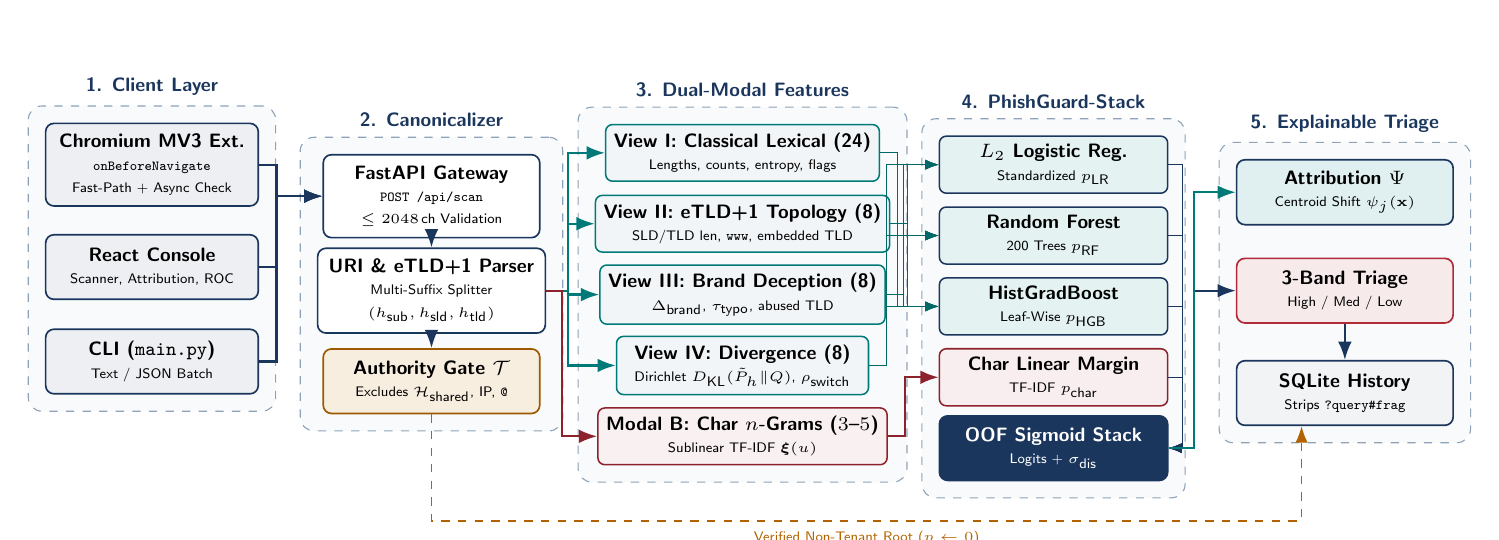
\begin{tikzpicture}[
    font=\scriptsize\sffamily,
    >=Latex,
    cbox/.style={draw=pgnavy, rounded corners=3pt, fill=white, minimum height=0.82cm, align=center, inner sep=4pt, line width=0.6pt},
    vbox/.style={draw=pgteal, rounded corners=2.5pt, fill=pgslate, minimum height=0.72cm, minimum width=3.2cm, align=center, inner sep=3pt, line width=0.55pt},
    mbox/.style={draw=pgnavy, rounded corners=2.5pt, fill=pgteal!10, minimum height=0.70cm, minimum width=2.9cm, align=center, inner sep=3pt, line width=0.55pt},
    sbg/.style={draw=pgborder, dashed, rounded corners=5pt, fill=pgslate!55, inner sep=6pt}
]
\node[cbox, fill=pgnavy!8, minimum width=2.7cm] (ext) at (0, 1.55) {\textbf{Chromium MV3 Ext.}\\{\tiny \texttt{onBeforeNavigate}}\\{\tiny Fast-Path + Async Check}};
\node[cbox, fill=pgnavy!8, minimum width=2.7cm] (ui)  at (0, 0.25) {\textbf{React Console}\\{\tiny Scanner, Attribution, ROC}};
\node[cbox, fill=pgnavy!8, minimum width=2.7cm] (cli) at (0, -0.95) {\textbf{CLI (\texttt{main.py})}\\{\tiny Text / JSON Batch}};
\begin{scope}[on background layer]
  \node[sbg, fit=(ext)(ui)(cli), label={[font=\scriptsize\bfseries\sffamily, text=pgnavy]above:1. Client Layer}] {};
\end{scope}

\node[cbox, minimum width=2.75cm] (api) at (3.55, 1.15) {\textbf{FastAPI Gateway}\\{\tiny \texttt{POST /api/scan}}\\{\tiny $\le 2048$\,ch Validation}};
\node[cbox, minimum width=2.75cm] (psl) at (3.55, -0.05) {\textbf{URI \& eTLD+1 Parser}\\{\tiny Multi-Suffix Splitter}\\{\tiny $(h_{\text{sub}}, h_{\text{sld}}, h_{\text{tld}})$}};
\node[cbox, fill=pgamber!12, draw=pgamber!80!black, minimum width=2.75cm] (trust) at (3.55, -1.20) {\textbf{Authority Gate $\mathcal{T}$}\\{\tiny Excludes $\mathcal{H}_{\text{shared}}$, IP, \texttt{@}}};
\begin{scope}[on background layer]
  \node[sbg, fit=(api)(psl)(trust), label={[font=\scriptsize\bfseries\sffamily, text=pgnavy]above:2. Canonicalizer}] {};
\end{scope}

\node[vbox] (v1) at (7.50, 1.70) {\textbf{View I: Classical Lexical (24)}\\{\tiny Lengths, counts, entropy, flags}};
\node[vbox] (v2) at (7.50, 0.80) {\textbf{View II: eTLD+1 Topology (8)}\\{\tiny SLD/TLD len, \texttt{www}, embedded TLD}};
\node[vbox] (v3) at (7.50, -0.10) {\textbf{View III: Brand Deception (8)}\\{\tiny $\Delta_{\text{brand}}$, $\tau_{\text{typo}}$, abused TLD}};
\node[vbox] (v4) at (7.50, -1.00) {\textbf{View IV: Divergence (8)}\\{\tiny Dirichlet $D_{\text{KL}}(\tilde{P}_h\|Q)$, $\rho_{\text{switch}}$}};
\node[vbox, draw=pgcrimson!80!black, fill=pgcrimson!7] (vc) at (7.50, -1.90) {\textbf{Modal B: Char $n$-Grams ($3$--$5$)}\\{\tiny Sublinear TF-IDF $\boldsymbol{\xi}(u)$}};
\begin{scope}[on background layer]
  \node[sbg, fit=(v1)(v2)(v3)(v4)(vc), label={[font=\scriptsize\bfseries\sffamily, text=pgnavy]above:3. Dual-Modal Features}] {};
\end{scope}

\node[mbox] (mlr)  at (11.45, 1.55) {\textbf{$L_2$ Logistic Reg.}\\{\tiny Standardized $p_{\text{LR}}$}};
\node[mbox] (mrf)  at (11.45, 0.65) {\textbf{Random Forest}\\{\tiny 200 Trees $p_{\text{RF}}$}};
\node[mbox] (mhgb) at (11.45, -0.25) {\textbf{HistGradBoost}\\{\tiny Leaf-Wise $p_{\text{HGB}}$}};
\node[mbox, draw=pgcrimson!80!black, fill=pgcrimson!8] (mch) at (11.45, -1.15) {\textbf{Char Linear Margin}\\{\tiny TF-IDF $p_{\text{char}}$}};
\node[cbox, fill=pgnavy, text=white, minimum width=2.9cm] (meta) at (11.45, -2.05) {\textbf{OOF Sigmoid Stack}\\{\tiny Logits + $\sigma_{\text{dis}}$}};
\begin{scope}[on background layer]
  \node[sbg, fit=(mlr)(mrf)(mhgb)(mch)(meta), label={[font=\scriptsize\bfseries\sffamily, text=pgnavy]above:4. PhishGuard-Stack}] {};
\end{scope}

\node[cbox, fill=pgteal!12, minimum width=2.75cm] (attr) at (15.15, 1.20) {\textbf{Attribution $\Psi$}\\{\tiny Centroid Shift $\psi_j(\mathbf{x})$}};
\node[cbox, fill=pgcrimson!10, draw=pgcrimson, minimum width=2.75cm] (band) at (15.15, -0.05) {\textbf{3-Band Triage}\\{\tiny High / Med / Low}};
\node[cbox, fill=pgnavy!6, minimum width=2.75cm] (db)   at (15.15, -1.35) {\textbf{SQLite History}\\{\tiny Strips \texttt{?query\#frag}}};
\begin{scope}[on background layer]
  \node[sbg, fit=(attr)(band)(db), label={[font=\scriptsize\bfseries\sffamily, text=pgnavy]above:5. Explainable Triage}] {};
\end{scope}

\draw[->, thick, pgnavy] (ext.east) -- ++(0.22,0) |- (api.west);
\draw[->, thick, pgnavy] (ui.east)  -- ++(0.22,0) |- (api.west);
\draw[->, thick, pgnavy] (cli.east) -- ++(0.22,0) |- (api.west);
\draw[->, thick, pgnavy] (api.south) -- (psl.north);
\draw[->, thick, pgnavy] (psl.south) -- (trust.north);
\foreach \v in {v1,v2,v3,v4} {
  \draw[->, thick, pgteal] (psl.east) -- ++(0.28,0) |- (\v.west);
  \draw[->, pgteal!85!black] (\v.east) -- ++(0.22,0) |- (mlr.west);
  \draw[->, pgteal!85!black] (\v.east) -- ++(0.22,0) |- (mrf.west);
  \draw[->, pgteal!85!black] (\v.east) -- ++(0.22,0) |- (mhgb.west);
}
\draw[->, thick, pgcrimson!80!black] (psl.east) -- ++(0.20,0) |- (vc.west);
\draw[->, thick, pgcrimson!80!black] (vc.east) -- ++(0.22,0) |- (mch.west);
\foreach \m in {mlr,mrf,mhgb,mch} {
  \draw[->, pgnavy] (\m.east) -- ++(0.18,0) |- (meta.east);
}
\draw[->, thick, pgnavy] (meta.east) -- ++(0.32,0) |- (band.west);
\draw[->, thick, pgteal] (meta.east) -- ++(0.32,0) |- (attr.west);
\draw[->, thick, pgnavy] (band.south) -- (db.north);
\draw[->, dashed, pgamber!90!black, line width=0.65pt] (trust.south) -- ++(0,-1.35) -| node[pos=0.25, below, font=\tiny\sffamily]{Verified Non-Tenant Root ($p \leftarrow 0$)} ([xshift=-0.55cm]db.south);
\end{tikzpicture}%
}
\caption{Proposed five-stage PhishGuard-Stack architecture enforcing strict zero-fetch URI screening.}
\label{fig:sysarch}
\end{figure}

\section{Single-Request Inference \& Browser Guard Flow}
Figure~\ref{fig:flow} depicts the server-side decision pipeline for each scan request, combined with the two-stage browser pre-navigation workflow. When a user clicks a link in Chromium, Stage~1 runs a synchronous JavaScript lexical rule check inside the Manifest~V3 service worker: blatantly malicious links (raw IP login URLs, \texttt{userinfo@} tricks, or nested brand tokens on abused TLDs) redirect immediately to \texttt{blocked.html} before network connection setup. Remaining URLs proceed to Stage~2, posting asynchronously to \texttt{POST /api/scan}; if the calibrated stack returns $p \ge 0.75$ (High Risk), the tab redirects upon response arrival ($\sim 14$\,ms).

\begin{figure}[htbp]
\centering
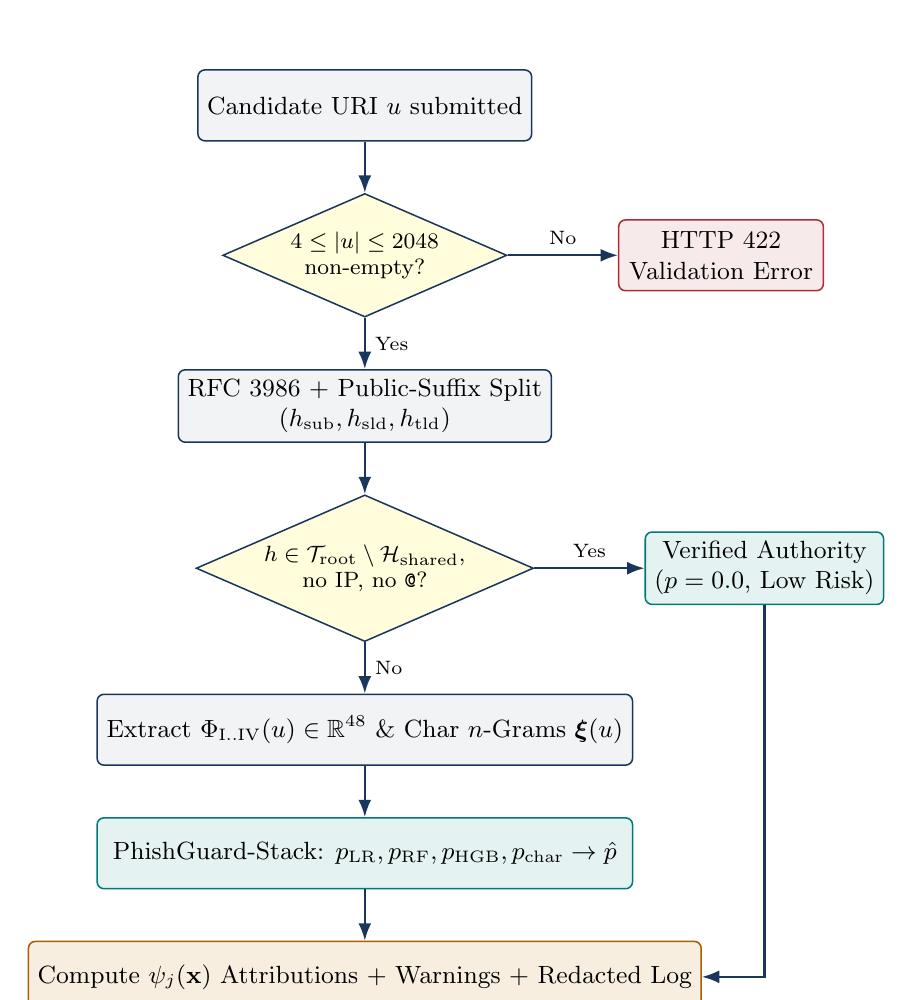
\begin{tikzpicture}[node distance=6.5mm]
  \node[box] (in) {Candidate URI $u$ submitted};
  \node[dec, below=of in] (val) {$4 \le |u| \le 2048$\\non-empty?};
  \node[boxr, right=14mm of val] (err) {HTTP 422\\Validation Error};
  \node[box, below=of val] (parse) {RFC 3986 + Public-Suffix Split\\$(h_{\text{sub}}, h_{\text{sld}}, h_{\text{tld}})$};
  \node[dec, below=of parse] (tr) {$h \in \mathcal{T}_{\text{root}} \setminus \mathcal{H}_{\text{shared}}$,\\no IP, no \texttt{@}?};
  \node[boxg, right=14mm of tr] (low) {Verified Authority\\($p=0.0$, Low Risk)};
  \node[box, below=of tr, minimum width=68mm] (dual) {Extract $\Phi_{\text{I..IV}}(u) \in \mathbb{R}^{48}$ \& Char $n$-Grams $\boldsymbol{\xi}(u)$};
  \node[boxg, below=of dual, minimum width=68mm] (stack) {PhishGuard-Stack: $p_{\text{LR}}, p_{\text{RF}}, p_{\text{HGB}}, p_{\text{char}} \to \hat{p}$};
  \node[boxo, below=of stack, minimum width=68mm] (out) {Compute $\psi_j(\mathbf{x})$ Attributions + Warnings + Redacted Log};
  \draw[arr] (in) -- (val);
  \draw[arr] (val) -- node[lab, above]{No} (err);
  \draw[arr] (val) -- node[lab, right]{Yes} (parse);
  \draw[arr] (parse) -- (tr);
  \draw[arr] (tr) -- node[lab, above]{Yes} (low);
  \draw[arr] (tr) -- node[lab, right]{No} (dual);
  \draw[arr] (dual) -- (stack);
  \draw[arr] (stack) -- (out);
  \draw[arr] (low) |- (out.east);
\end{tikzpicture}
\caption{Server-side validation, shared-host-aware authority gating, dual-modal stacking, and attribution workflow.}
\label{fig:flow}
\end{figure}

\section{Calibrated Three-Band Operational Triage}
Binary labels alone force an all-or-nothing trade-off between blocking benign documentation pages and missing subtle phishing links. Because PhishGuard-Stack produces well-calibrated posterior probabilities ($\text{ECE}=0.0188$), we map $\hat{p} \in [0,1]$ into three operational risk bands (Figure~\ref{fig:bands}): \textbf{Low Risk} ($\hat{p} < 0.45$, normal navigation), \textbf{Medium Risk} ($0.45 \le \hat{p} < 0.75$, amber caution badge/advisory banner), and \textbf{High Risk} ($\hat{p} \ge 0.75$, full-page interstitial warning with session override), while binary classification uses threshold $0.50$.

\begin{figure}[htbp]
\centering
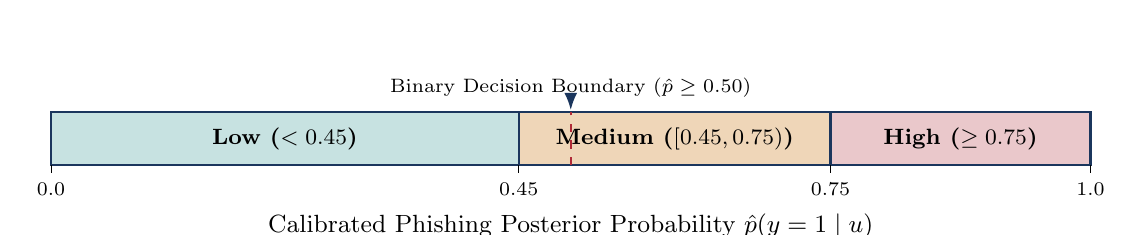
\begin{tikzpicture}[x=13.2cm]
  \fill[pgteal!22]    (0,0) rectangle (0.45,0.68);
  \fill[pgamber!28]   (0.45,0) rectangle (0.75,0.68);
  \fill[pgcrimson!26] (0.75,0) rectangle (1,0.68);
  \draw[pgnavy, thick] (0,0) rectangle (1,0.68);
  \draw[pgnavy, thick] (0.45,0) -- (0.45,0.68);
  \draw[pgnavy, thick] (0.75,0) -- (0.75,0.68);
  \node[font=\footnotesize\bfseries] at (0.225,0.34) {Low ($<0.45$)};
  \node[font=\footnotesize\bfseries] at (0.600,0.34) {Medium ($[0.45,0.75)$)};
  \node[font=\footnotesize\bfseries] at (0.875,0.34) {High ($\ge 0.75$)};
  \foreach \x/\l in {0/0.0,0.45/0.45,0.75/0.75,1/1.0}
    \draw (\x,0) -- (\x,-0.10) node[below, font=\scriptsize] {\l};
  \draw[dashed, thick, pgcrimson] (0.5,0) -- (0.5,0.68);
  \node[font=\scriptsize, align=center] at (0.5,0.98) {Binary Decision Boundary ($\hat{p} \ge 0.50$)};
  \draw[arr] (0.5,0.84) -- (0.5,0.70);
  \node[font=\small] at (0.5,-0.78) {Calibrated Phishing Posterior Probability $\hat{p}(y=1 \mid u)$};
\end{tikzpicture}
\caption{Three-band operational triage over calibrated stacking probabilities.}
\label{fig:bands}
\end{figure}

% =========================== CHAPTER 5 ==================================
\chapter{Formal Mathematical Model}

\section{Set-Theoretic System Definition}
We define PhishGuard-Stack formally as a deterministic seven-tuple screening automaton:
\begin{equation}
\mathcal{S} = \langle \mathcal{U},\, \mathcal{T},\, \Phi,\, \mathcal{G}_{\text{char}},\, \mathcal{M},\, \mathcal{C},\, \Psi \rangle,
\label{eq:systuple}
\end{equation}
where $\mathcal{U} \subseteq \Sigma^{\le 2048}$ is the bounded URI input space; $\mathcal{T}: \mathcal{U} \to \{0,1\}$ is the shared-host-aware authority predicate; $\Phi: \mathcal{U} \to \mathbb{R}^{48}$ extracts four structured feature views $\Phi(u) = [\Phi_{\text{I}} \,\|\, \Phi_{\text{II}} \,\|\, \Phi_{\text{III}} \,\|\, \Phi_{\text{IV}}]^\top$; $\mathcal{G}_{\text{char}}: \mathcal{U} \to \mathbb{R}^{V}$ computes normalized sublinear character $n$-gram TF-IDF features ($V \le 22{,}000$); $\mathcal{M} = \{f_{\text{LR}}, f_{\text{RF}}, f_{\text{HGB}}, f_{\text{char}}\}$ is the heterogeneous learner ensemble; $\mathcal{C}: [0,1]^4 \to [0,1]$ is the out-of-fold sigmoid meta-calibrator; and $\Psi: \mathbb{R}^{48} \to \mathbb{R}^{48}$ maps inputs to signed instance-level feature attributions.

\section{Public-Suffix-Aware URI Decomposition (View II)}
Given lowercased, port-stripped host $h$ with dot-separated labels $(l_1, \dots, l_k)$ and our 52-entry multi-label effective suffix registry $\mathcal{E}_2$ (covering \texttt{.co.in}, \texttt{.ac.in}, \texttt{.gov.in}, \texttt{.co.uk}, \texttt{.com.au}, \texttt{.co.jp}, etc.), canonical decomposition $(h_{\text{sub}}, h_{\text{sld}}, h_{\text{tld}})$ is given by:
\begin{equation}
(h_{\text{sub}}, h_{\text{sld}}, h_{\text{tld}}) =
\begin{cases}
(l_{1..k-3},\; l_{k-2},\; l_{k-1}.l_k), & \text{if } k \ge 3 \land l_{k-1}.l_k \in \mathcal{E}_{2}, \\
(l_{1..k-2},\; l_{k-1},\; l_k), & \text{if } k \ge 2 \land l_{k-1}.l_k \notin \mathcal{E}_{2}.
\end{cases}
\label{eq:rep_etld}
\end{equation}
The registrable group identifier used for anti-leakage dataset partitioning is $g(u) = h_{\text{sld}}.h_{\text{tld}}$ (or tenant-qualified $l_{\text{tenant}}.h_{\text{sld}}.h_{\text{tld}}$ when $h$ suffixes $\mathcal{H}_{\text{shared}}$).

\section[Brand-Domain Spoofing Asymmetry \& Typosquatting]{Brand-Domain Spoofing Asymmetry and Typosquatting (View III)}
Let $\Gamma(t)$ denote canonicalized leetspeak/homoglyph variants of token $t$ (\texttt{0}$\to$\texttt{o}, \texttt{1}$\to$\texttt{l}/\texttt{i}, \texttt{3}$\to$\texttt{e}, \texttt{4}$\to$\texttt{a}, \texttt{5}$\to$\texttt{s}, \texttt{rn}$\to$\texttt{m}, \texttt{vv}$\to$\texttt{w}), and let $\mathcal{B}$ be our lexicon of 48 target brands where each brand $b \in \mathcal{B}$ maps to authorized owner SLD set $\Omega(b)$. Length-gated similarity $\kappa(t,b)$ is defined via bounded Levenshtein distance $d_{\text{lev}}$:
\begin{equation}
\kappa(t, b) = \max_{v \in \Gamma(t)}
\begin{cases}
1.00, & \text{if } t = b, \\
0.96, & \text{if } t \neq b \land v = b, \\
1 - \dfrac{d_{\text{lev}}(v, b)}{\max(|v|, |b|)}, & \text{if } d_{\text{lev}}(v,b) \le \delta(|v|,|b|), \\
0, & \text{otherwise},
\end{cases}
\end{equation}
with $\delta(\ell_1,\ell_2) = 2$ for $\min(\ell_1,\ell_2) \ge 8$, $1$ for $5 \le \min(\ell_1,\ell_2) < 8$, and $0$ otherwise. Setting effective owner $\tilde{o}(u) = \varnothing$ if $h \in \mathcal{H}_{\text{shared}}$ else $h_{\text{sld}}$, \textbf{Brand-Domain Spoofing Divergence} $\Delta_{\text{brand}}(u)$ and \textbf{SLD Typosquatting Proximity} $\tau_{\text{typo}}(h_{\text{sld}})$ are:
\begin{align}
\Delta_{\text{brand}}(u) &= \max_{b \in \mathcal{B} \,:\, \tilde{o}(u) \notin \Omega(b)} \max\!\left( \max_{t \in \mathcal{W}_{\text{host}}} \kappa(t,b),\; 0.90 \!\!\max_{t \in \mathcal{W}_{\text{path}}} \mathbb{I}[\kappa(t,b) \ge 0.96]\kappa(t,b) \right), \\
\tau_{\text{typo}}(h_{\text{sld}}) &= \max_{\substack{b \in \mathcal{B},\; \tilde{o}(u) \notin \Omega(b) \\ c \in \{h_{\text{sld}},\, h_{\text{sld}}^{-}\} \,:\, c \neq b \lor \text{`-'}\in h_{\text{sld}}}} \kappa(c, b).
\end{align}

\section{Dirichlet-Smoothed KL-Divergence \& Morphology (View IV)}
To measure how strongly hostname characters deviate from natural English domain priors $Q$ without penalizing short benign acronyms, we strip leading \texttt{www.} to obtain $h_{\text{core}}$ of alphanumeric length $n$ and apply Dirichlet smoothing with concentration $\alpha = 5.0$:
\begin{equation}
\tilde{P}_{h}(a) = \frac{c_a + \alpha Q(a)}{n + \alpha}, \qquad D_{\text{KL}}\!\left(\tilde{P}_h \,\middle\|\, Q\right) = \sum_{a \in \mathcal{A}_{36}} \tilde{P}_h(a) \log_2 \frac{\tilde{P}_h(a)}{Q(a)}.
\end{equation}
Character-class switching rate $\rho_{\text{switch}}(h)$ quantifies rapid alternation across letter, digit, and punctuation classes:
\begin{equation}
\rho_{\text{switch}}(h) = \frac{1}{\max(|h|-1, 1)} \sum_{i=1}^{|h|-1} \mathbb{I}\!\left[\pi(h_i) \neq \pi(h_{i+1})\right].
\end{equation}
Table~\ref{tab:all48} lists all 48 features across Views~I--IV.

\begin{table}[htbp]
\caption[Complete 48-Feature Multi-View Schema]{Complete 48-Feature Multi-View Schema Extracted in \texttt{feature\_extractor.py}}
\label{tab:all48}
\centering
\scriptsize
\renewcommand{\arraystretch}{1.14}
\begin{tabular}{p{2.2cm}cp{9.8cm}}
\toprule
\textbf{Feature View} & \textbf{Count} & \textbf{Feature Identifiers} \\
\midrule
\textbf{View I:} Classical Lexical Baseline & 24 & \texttt{url\_length}, \texttt{hostname\_length}, \texttt{path\_length}, \texttt{query\_length}, \texttt{dot\_count}, \texttt{hyphen\_count}, \texttt{underscore\_count}, \texttt{slash\_count}, \texttt{question\_mark\_count}, \texttt{equal\_count}, \texttt{ampersand\_count}, \texttt{at\_symbol}, \texttt{double\_slash\_redirect}, \texttt{subdomain\_count}, \texttt{digit\_count}, \texttt{special\_char\_count}, \texttt{suspicious\_keyword\_count}, \texttt{https}, \texttt{ip\_host}, \texttt{is\_shortener}, \texttt{hostname\_entropy}, \texttt{has\_port}, \texttt{has\_fragment}, \texttt{tld\_in\_path} \\
\midrule
\textbf{View II:} eTLD+1 Topology \emph{(Novel)} & 8 & \texttt{sld\_length}, \texttt{tld\_length}, \texttt{has\_www}, \texttt{www\_misplaced}, \texttt{path\_depth}, \texttt{longest\_token\_length}, \texttt{tld\_in\_subdomain}, \texttt{host\_url\_ratio} \\
\midrule
\textbf{View III:} Brand Deception \emph{(Novel)} & 8 & \texttt{brand\_spoof\_score} ($\Delta_{\text{brand}}$), \texttt{sld\_typosquat\_score} ($\tau_{\text{typo}}$), \texttt{brand\_in\_subdomain}, \texttt{host\_keyword\_count}, \texttt{suspicious\_tld}, \texttt{free\_hosting\_host}, \texttt{punycode\_idn}, \texttt{digits\_in\_sld} \\
\midrule
\textbf{View IV:} Divergence \& Morph.\ \emph{(Novel)} & 8 & \texttt{path\_entropy}, \texttt{hostname\_kl\_divergence} ($D_{\text{KL}}$), \texttt{char\_transition\_rate} ($\rho_{\text{switch}}$), \texttt{digit\_ratio\_host}, \texttt{vowel\_ratio}, \texttt{max\_consonant\_run}, \texttt{uppercase\_ratio}, \texttt{percent\_encoding\_count} \\
\bottomrule
\end{tabular}
\end{table}

\section{Dual-Modal Out-of-Fold Stacking \& Centroid Attribution}
Modal~B transforms raw URL strings into $L_2$-normalized sublinear TF-IDF character $n$-gram vectors $\boldsymbol{\xi}(u)$ ($3 \le n \le 5$, $V \le 22{,}000$). Partitioning training data into $K=5$ registrable-domain-disjoint folds, out-of-fold base posteriors $\mathbf{p} = [p_{\text{LR}}, p_{\text{RF}}, p_{\text{HGB}}, p_{\text{char}}]^\top$, clipped log-odds $\ell(\mathbf{p})$, and epistemic standard deviation $\sigma_{\text{dis}}(u) = \text{std}(\mathbf{p})$ form meta-vector $\mathbf{z}(u) = [\mathbf{p}^\top, \ell(\mathbf{p})^\top, \sigma_{\text{dis}}]^\top \in \mathbb{R}^9$. The calibrated posterior and benign-centroid instance attribution $\psi_j(\mathbf{x})$ are:
\begin{align}
\hat{p}(y=1 \mid u) &= \sigma\!\left(\boldsymbol{\beta}^\top \mathbf{z}(u) + \beta_0\right), \\
\psi_j(\mathbf{x}) &= \left(0.45\,\tilde{w}_j^{\text{LR}} + 0.55\,\tilde{g}_j^{\text{RF}} s_j\right) \cdot \text{clip}\!\left(\frac{x_j - \mu_j^{(0)}}{\sigma_j}, -6, 6\right).
\end{align}
Asymptotic per-URL extraction and inference time is $\mathcal{O}(|u| + |\mathcal{B}|\cdot|h_{\text{sld}}| + (T_{\text{RF}}+T_{\text{HGB}})D)$, which is bounded by a small constant for $|u| \le 2048$.

% =========================== CHAPTER 6 ==================================
\chapter{System Implementation}

\section{Backend ML and Service Modules}
The Python backend under \texttt{phishguard/backend/app/} separates feature math, ensemble estimation, API validation, and persistence cleanly:
\begin{itemize}
\item \textbf{\texttt{ml/\allowbreak feature\_\allowbreak extractor.py}:} Implements \texttt{split\_\allowbreak registrable\_\allowbreak domain()}, homoglyph canonicalization, length-gated Levenshtein brand matching with \texttt{@lru\_\allowbreak cache}, Dirichlet-smoothed KL-divergence, and \texttt{extract\_\allowbreak features()} returning all 48 deterministic features.
\item \textbf{\texttt{ml/ensemble.py}:} Implements \texttt{PhishGuard\allowbreak StackClassifier} (\texttt{Base\allowbreak Estimator}, \texttt{Classifier\allowbreak Mixin}), orchestrating 5-fold \texttt{Stratified\allowbreak GroupKFold} out-of-fold meta-training across $L_2$ Logistic Regression, 200-tree Balanced Random Forest, 260-iteration HistGradientBoosting, and 22,000-feature Character $n$-Gram Logistic Regression, plus \texttt{explain\_\allowbreak instance()}. Post-fit, Random Forest is switched to \texttt{n\_jobs=1} to eliminate single-row thread-spawning overhead.
\item \textbf{\texttt{ml/model\_service.py} \& \texttt{api/routes.py}:} Exposes \texttt{GET /api/health}, \texttt{POST /api/\allowbreak scan}, \texttt{GET /api/\allowbreak model/\allowbreak metrics}, \texttt{GET /api/\allowbreak history}, and \texttt{DELETE /api/\allowbreak history} with Pydantic v2 schemas and query-redacted SQLite storage.
\end{itemize}

\section{Analyst Web Console, CLI, and Manifest V3 Extension}
The React/TypeScript web application (\texttt{phishguard/frontend/}) provides an interactive Scanner view displaying the calibrated risk gauge, ensemble sub-model breakdown, top signed feature attributions, and plain-English warnings, alongside a live Evaluation Dashboard visualizing domain-disjoint metrics, confusion matrices, and baseline comparisons. Terminal users can audit individual or scripted URLs via \texttt{python main.py <url> -{}-format json -{}-verbose}. Inside \texttt{phishguard/extension/}, the Manifest~V3 service worker (\texttt{background.js}) hooks \texttt{chrome.webNavigation.onBeforeNavigate} to pair instant rule-based blocking with local FastAPI escalation.

% =========================== CHAPTER 7 ==================================
\chapter[Experimental Evaluation and Comparative Results]{Experimental Evaluation, Justification and Comparative Results}

\section{Real-World Benchmark Corpora and Anti-Leakage Split}
All synthetic datasets were eliminated. Primary training and evaluation use the peer-reviewed \textbf{Hannousse and Yahiouche (2021)} benchmark \cite{hannousse2021} (Mendeley DOI: \texttt{10.17632/\allowbreak c2gw7fy2j4.3}), containing \textbf{$11{,}429$ unique real URLs} ($5{,}715$ legitimate, $5{,}714$ phishing; $44.5\%$ vs.\ $33.3\%$ HTTPS) across \textbf{$7{,}188$ unique registrable domains}. Using 5-fold \texttt{Stratified\allowbreak GroupKFold} grouped by canonical registrable domain $g(u)$, Fold~1 forms the held-out test set ($9{,}143$ training URLs across $5{,}752$ domains; $2{,}286$ test URLs across $1{,}436$ unseen domains; \textbf{exact domain overlap $= 0$}). External zero-shot generalization is evaluated on \textbf{$10{,}000$ unseen Ebbu2017 URLs} \cite{sahingoz2019} and \textbf{$300$ live 2026 OpenPhish zero-day URLs} ($53.3\%$ HTTPS).

\section{Quantitative Comparison Across Nine ML Classifiers}
Table~\ref{tab:rep_models} reports performance across nine classifiers on the held-out domain-disjoint split ($N_{\text{test}}=2{,}286$). PhishGuard-Stack achieves the highest accuracy ($93.00\%$), recall ($94.14\%$), F1-score ($0.9308$), ROC-AUC ($0.9833$), and PR-AUC ($0.9855$), while achieving the lowest Brier calibration loss ($0.0494$) and Expected Calibration Error ($0.0188$).

\begin{table}[htbp]
\caption{Comparison of Nine Classifiers on Held-Out Domain-Disjoint Split ($N=2{,}286$)}
\label{tab:rep_models}
\centering
\scriptsize
\renewcommand{\arraystretch}{1.16}
\begin{tabular}{lcccccccc}
\toprule
\textbf{Classifier} & \textbf{Acc.} & \textbf{Prec.} & \textbf{Rec.} & \textbf{F1} & \textbf{AUC} & \textbf{FPR} & \textbf{Brier} & \textbf{ECE} \\
\midrule
Gaussian Naive Bayes (48f) & 0.7423 & \textbf{0.9439} & 0.5153 & 0.6667 & 0.8986 & \textbf{0.0306} & 0.2544 & 0.2553 \\
Decision Tree (48f) & 0.8132 & 0.7850 & 0.8626 & 0.8220 & 0.8695 & 0.2362 & 0.1453 & 0.1010 \\
$K$-Nearest Neighbors (48f) & 0.8285 & 0.8493 & 0.7988 & 0.8233 & 0.9065 & 0.1417 & 0.1246 & 0.0552 \\
Calibrated Linear SVM (48f) & 0.8469 & 0.8451 & 0.8495 & 0.8473 & 0.9368 & 0.1557 & 0.1014 & 0.0327 \\
$L_2$ Logistic Regression (48f) & 0.8486 & 0.8486 & 0.8486 & 0.8486 & 0.9362 & 0.1514 & 0.1017 & 0.0312 \\
MLP Neural Network (48f) & 0.8753 & 0.8540 & 0.9055 & 0.8790 & 0.9574 & 0.1549 & 0.0848 & 0.0391 \\
Balanced Random Forest (48f) & 0.8832 & 0.8724 & 0.8976 & 0.8849 & 0.9567 & 0.1312 & 0.0901 & 0.0811 \\
HistGradientBoosting (48f) & 0.8972 & 0.8847 & 0.9134 & 0.8988 & 0.9663 & 0.1190 & 0.0725 & 0.0259 \\
\midrule
\textbf{PhishGuard-Stack (Proposed)} & \textbf{0.9300} & 0.9204 & \textbf{0.9414} & \textbf{0.9308} & \textbf{0.9833} & 0.0814 & \textbf{0.0494} & \textbf{0.0188} \\
\bottomrule
\end{tabular}
\end{table}

\section[Comparison of Proposed vs. Existing Lexical Systems]{Comparison of Proposed System vs.\ Existing Lexical Frameworks}
Table~\ref{tab:rep_existing} benchmarks PhishGuard-Stack against five re-implemented lexical systems on the identical domain-disjoint split, accompanied by continuity-corrected McNemar $\chi^2_{\text{cc}}$ statistics. Compared to the 24-feature Sahingoz / PhishGuard-v1 baseline ($87.18\%$), our proposed architecture improves accuracy by \textbf{$+5.82$ percentage points} ($n_{10}=201$ vs.\ $n_{01}=68$, $\chi^2_{\text{cc}}=64.77, p < 10^{-15}$) and cuts false positives from $156$ down to $93$ ($-40.4\%$).

\begin{table}[htbp]
\caption{Quantitative Comparison Against Existing Lexical URL Detection Systems}
\label{tab:rep_existing}
\centering
\scriptsize
\renewcommand{\arraystretch}{1.16}
\begin{tabular}{p{4.7cm}ccccccc}
\toprule
\textbf{System / Lexical Framework} & \textbf{Acc.} & \textbf{Prec.} & \textbf{Rec.} & \textbf{F1} & \textbf{AUC} & \textbf{FPR} & \textbf{McNemar $\chi^2_{\text{cc}}$} \\
\midrule
Static Browser Heuristic Rules (9f) & 0.5459 & 1.0000 & 0.0919 & 0.1683 & 0.7541 & 0.0000 & $865.1$ ($p<10^{-16}$) \\
Garera et al.\ \cite{garera2007} (8f + LR) & 0.7038 & 0.7995 & 0.5442 & 0.6476 & 0.7385 & 0.1365 & $392.4$ ($p<10^{-16}$) \\
Feroz \& Mengel \cite{feroz2015} (15f + RF) & 0.8495 & 0.8383 & 0.8661 & 0.8520 & 0.9184 & 0.1671 & $100.9$ ($p<10^{-16}$) \\
Sahingoz / PhishGuard-v1 \cite{sahingoz2019} (24f + RF) & 0.8718 & 0.8657 & 0.8801 & 0.8729 & 0.9359 & 0.1365 & $64.77$ ($p<10^{-15}$) \\
Character $n$-Gram Linear Baseline & 0.9125 & 0.9132 & 0.9116 & 0.9124 & 0.9728 & 0.0866 & $12.89$ ($p=0.0003$) \\
\midrule
\textbf{PhishGuard-Stack (Proposed Dual-Modal)} & \textbf{0.9300} & \textbf{0.9204} & \textbf{0.9414} & \textbf{0.9308} & \textbf{0.9833} & \textbf{0.0814} & \textbf{Reference} \\
\bottomrule
\end{tabular}
\end{table}

\section{Confusion Matrix, ROC, and Calibration Diagnostics}
Figures~\ref{fig:rep_cm} and~\ref{fig:rep_roc} illustrate the held-out domain-disjoint confusion matrix ($\text{TN}=1{,}050$, $\text{FP}=93$, $\text{FN}=67$, $\text{TP}=1{,}076$), ROC curves, and 10-bin reliability calibration plot.

\begin{figure}[htbp]
\centering
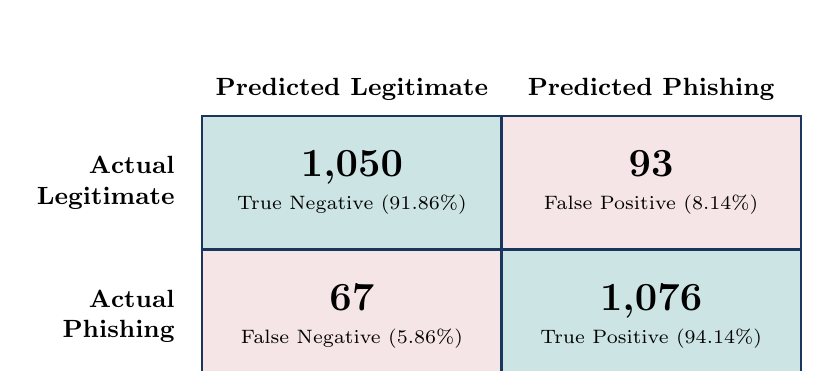
\begin{tikzpicture}[x=3.8cm, y=1.7cm]
  \fill[pgteal!20]    (0,1) rectangle (1,2);
  \fill[pgcrimson!12] (1,1) rectangle (2,2);
  \fill[pgcrimson!12] (0,0) rectangle (1,1);
  \fill[pgteal!20]    (1,0) rectangle (2,1);
  \draw[pgnavy, thick] (0,0) rectangle (2,2);
  \draw[pgnavy, thick] (1,0) -- (1,2);
  \draw[pgnavy, thick] (0,1) -- (2,1);
  \node[align=center] at (0.5,1.5) {{\Large\bfseries 1,050}\\{\scriptsize True Negative (91.86\%)}};
  \node[align=center] at (1.5,1.5) {{\Large\bfseries 93}\\{\scriptsize False Positive (8.14\%)}};
  \node[align=center] at (0.5,0.5) {{\Large\bfseries 67}\\{\scriptsize False Negative (5.86\%)}};
  \node[align=center] at (1.5,0.5) {{\Large\bfseries 1,076}\\{\scriptsize True Positive (94.14\%)}};
  \node[above, font=\small\bfseries] at (0.5,2.04) {Predicted Legitimate};
  \node[above, font=\small\bfseries] at (1.5,2.04) {Predicted Phishing};
  \node[left, font=\small\bfseries, align=right] at (-0.06,1.5) {Actual\\Legitimate};
  \node[left, font=\small\bfseries, align=right] at (-0.06,0.5) {Actual\\Phishing};
\end{tikzpicture}
\caption{Confusion matrix of PhishGuard-Stack on $2{,}286$ unseen-domain test URLs.}
\label{fig:rep_cm}
\end{figure}

\begin{figure}[htbp]
\centering
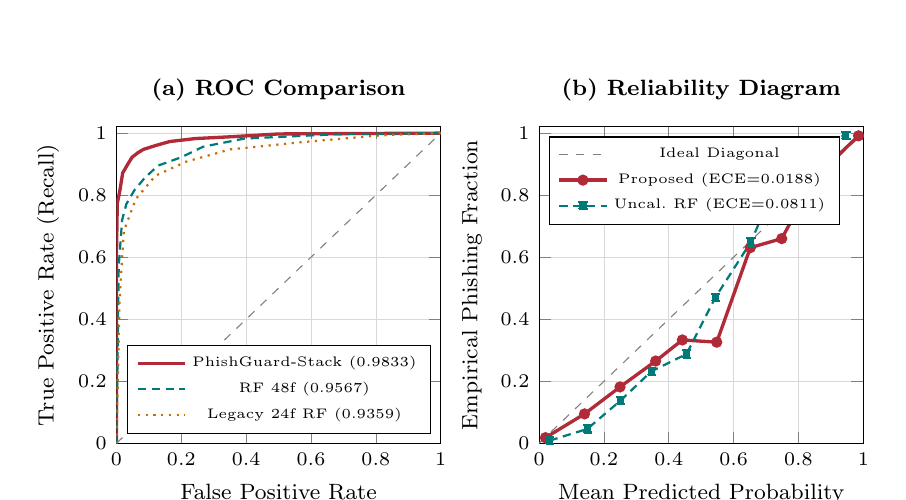
\begin{tikzpicture}
\begin{axis}[
    name=p1,
    width=0.47\textwidth,
    height=5.6cm,
    xlabel={False Positive Rate},
    ylabel={True Positive Rate (Recall)},
    title={\textbf{(a) ROC Comparison}},
    xmin=0, xmax=1, ymin=0, ymax=1.02,
    grid=both,
    grid style={line width=0.2pt, draw=gray!30},
    legend pos=south east,
    legend style={font=\tiny},
    label style={font=\footnotesize},
    tick label style={font=\scriptsize},
    title style={font=\footnotesize}
]
\addplot[pgcrimson, very thick] coordinates {
  (0.0,0.0) (0.0,0.6063) (0.0026,0.7734) (0.0105,0.8145) (0.0192,0.8714) (0.0341,0.8985)
  (0.0481,0.9221) (0.0665,0.9370) (0.0831,0.9475) (0.1199,0.9598) (0.1645,0.9729)
  (0.2432,0.9825) (0.3587,0.9886) (0.5004,0.9974) (1.0,1.0)
};
\addlegendentry{PhishGuard-Stack (0.9833)}
\addplot[pgteal, thick, densely dashed] coordinates {
  (0.0,0.0) (0.0070,0.5722) (0.0175,0.7200) (0.0306,0.7717) (0.0551,0.8154)
  (0.0857,0.8539) (0.1277,0.8950) (0.1995,0.9221) (0.2677,0.9563) (0.3946,0.9825)
  (0.6824,0.9965) (1.0,1.0)
};
\addlegendentry{RF 48f (0.9567)}
\addplot[pgamber, thick, dotted] coordinates {
  (0.0,0.0) (0.0096,0.4584) (0.0227,0.6842) (0.0595,0.7874) (0.1199,0.8626)
  (0.2152,0.9081) (0.3508,0.9475) (0.5661,0.9703) (0.8171,0.9930) (1.0,1.0)
};
\addlegendentry{Legacy 24f RF (0.9359)}
\addplot[gray, thin, dashed] coordinates {(0,0) (1,1)};
\end{axis}

\begin{axis}[
    at={(p1.east)},
    anchor=west,
    xshift=1.25cm,
    width=0.47\textwidth,
    height=5.6cm,
    xlabel={Mean Predicted Probability},
    ylabel={Empirical Phishing Fraction},
    title={\textbf{(b) Reliability Diagram}},
    xmin=0, xmax=1, ymin=0, ymax=1.02,
    grid=both,
    grid style={line width=0.2pt, draw=gray!30},
    legend pos=north west,
    legend style={font=\tiny},
    label style={font=\footnotesize},
    tick label style={font=\scriptsize},
    title style={font=\footnotesize}
]
\addplot[gray, thin, dashed] coordinates {(0,0) (1,1)};
\addlegendentry{Ideal Diagonal}
\addplot[pgcrimson, very thick, mark=*, mark size=1.4pt] coordinates {
  (0.0197,0.0182) (0.1402,0.0949) (0.2497,0.1818) (0.3596,0.2653) (0.4420,0.3333)
  (0.5480,0.3261) (0.6517,0.6308) (0.7485,0.6600) (0.8504,0.8571) (0.9854,0.9913)
};
\addlegendentry{Proposed (ECE=0.0188)}
\addplot[pgteal, thick, densely dashed, mark=square*, mark size=1.3pt] coordinates {
  (0.0325,0.0087) (0.1487,0.0464) (0.2508,0.1374) (0.3463,0.2320) (0.4548,0.2879)
  (0.5434,0.4697) (0.6531,0.6489) (0.7545,0.8918) (0.8510,0.9681) (0.9463,0.9926)
};
\addlegendentry{Uncal.\ RF (ECE=0.0811)}
\end{axis}
\end{tikzpicture}
\caption{Held-out domain-disjoint ROC curves and 10-bin calibration curves.}
\label{fig:rep_roc}
\end{figure}

\section{Ablation Study, 5-Fold CV, and Zero-Day OOD Generalization}
Tables~\ref{tab:rep_ablation} and~\ref{tab:rep_cv_ood} summarize our 7-stage ablation study, 5-fold registrable-domain-disjoint cross-validation ($92.69\% \pm 0.40\%$ accuracy), $1{,}000$-bootstrap $95\%$ confidence intervals, and zero-shot cross-dataset evaluation on Sahingoz Ebbu2017 ($N=10{,}000$, $92.25\%$ accuracy vs.\ $84.57\%$ legacy baseline) and live 2026 OpenPhish URLs ($90.33\%$ zero-day recall). Figure~\ref{fig:rep_imp} plots the top 10 hybrid tabular attribution sensitivities, confirming that \texttt{https} ($0.0104$, rank 31) no longer dominates classification.

\begin{table}[htbp]
\caption{Seven-Stage Feature and Stacking Ablation Study ($N_{\text{test}}=2{,}286$)}
\label{tab:rep_ablation}
\centering
\footnotesize
\begin{tabular}{p{8.2cm}cccc}
\toprule
\textbf{Ablation Stage} & \textbf{Acc.} & \textbf{F1} & \textbf{ROC-AUC} & \textbf{Brier} \\
\midrule
A0: View I (24 Classical Lexical) + Logistic Regression & 0.7625 & 0.7376 & 0.8280 & 0.1659 \\
A1: View I (24 Classical Lexical) + Random Forest & 0.8679 & 0.8696 & 0.9344 & 0.1037 \\
A2: + View II (Public-Suffix Topology \& Placement, 32f) & 0.8657 & 0.8710 & 0.9503 & 0.0939 \\
A3: + View III (Homoglyph Brand Spoofing \& Host Abuse, 40f) & 0.8714 & 0.8748 & 0.9521 & 0.0921 \\
A4: + View IV (Dirichlet KL-Divergence \& Morphology, 48f) & 0.8600 & 0.8651 & 0.9542 & 0.0923 \\
A5: + Tabular Out-of-Fold Calibrated Stack (LR+RF+HGB, 48f) & 0.8950 & 0.8969 & 0.9668 & 0.0731 \\
\textbf{A6: + Subword Char $n$-Gram Dual-Modal PhishGuard-Stack} & \textbf{0.9300} & \textbf{0.9308} & \textbf{0.9833} & \textbf{0.0494} \\
\bottomrule
\end{tabular}
\end{table}

\begin{table}[htbp]
\caption[5-Fold Domain-Disjoint CV and Zero-Shot OOD Benchmarks]{5-Fold Domain-Disjoint Cross-Validation, Bootstrap 95\% CIs, and Zero-Shot OOD Benchmarks}
\label{tab:rep_cv_ood}
\centering
\scriptsize
\renewcommand{\arraystretch}{1.15}
\resizebox{\textwidth}{!}{%
\begin{tabular}{p{5.8cm}ccccc}
\toprule
\textbf{Evaluation Regime} & \textbf{Acc.} & \textbf{Prec.} & \textbf{Rec.} & \textbf{F1} & \textbf{ROC-AUC} \\
\midrule
Hannousse 5-Fold Domain-Disjoint Mean $\pm$ SD ($N=11{,}429$) & $0.9269 \pm 0.0040$ & $0.9284 \pm 0.0086$ & $0.9251 \pm 0.0096$ & $0.9267 \pm 0.0041$ & $0.9795 \pm 0.0044$ \\
Held-Out Test 95\% Bootstrap CI ($1{,}000$ resamples) & $[0.9204, 0.9409]$ & $[0.9054, 0.9365]$ & $[0.9272, 0.9549]$ & $[0.9207, 0.9420]$ & $[0.9794, 0.9875]$ \\
\midrule
OOD Ebbu2017 Unseen Domains ($N=10{,}000$) --- Legacy 24f RF & 0.8457 & 0.8033 & 0.9156 & 0.8558 & 0.9344 \\
\textbf{OOD Ebbu2017 Unseen Domains ($N=10{,}000$) --- Proposed} & \textbf{0.9225} & \textbf{0.8997} & \textbf{0.9510} & \textbf{0.9246} & \textbf{0.9813} \\
\midrule
Live 2026 OpenPhish + HTTPS Benign ($N=600$) --- Legacy 24f RF & 0.8483 & 0.8317 & 0.8733 & 0.8520 & 0.9241 \\
\textbf{Live 2026 OpenPhish + HTTPS Benign ($N=600$) --- Proposed} & \textbf{0.9050} & \textbf{0.9064} & \textbf{0.9033} & \textbf{0.9048} & \textbf{0.9661} \\
\bottomrule
\end{tabular}%
}
\end{table}

\begin{figure}[htbp]
\centering
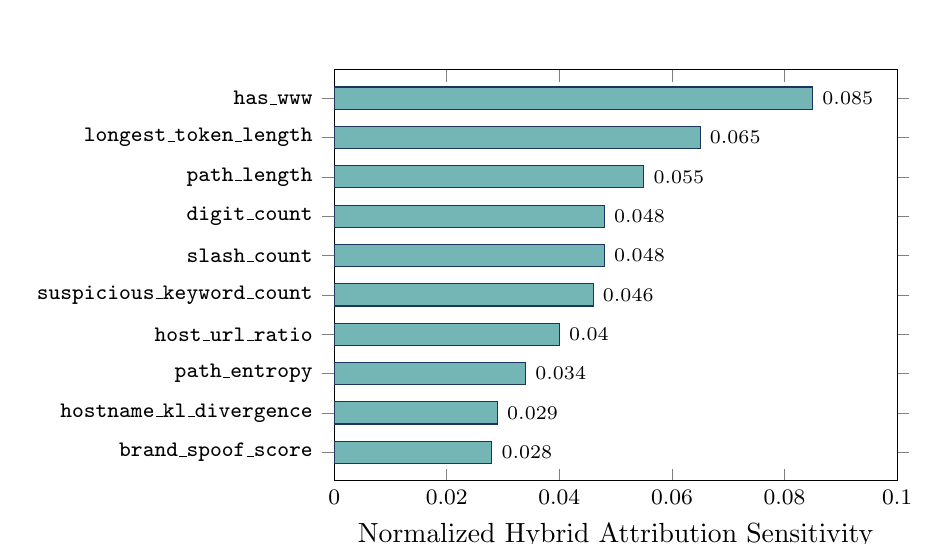
\begin{tikzpicture}
\begin{axis}[
    xbar,
    width=0.72\textwidth,
    height=6.8cm,
    bar width=8pt,
    xmin=0, xmax=0.10,
    xtick={0,0.02,0.04,0.06,0.08,0.10},
    xticklabel style={/pgf/number format/.cd, fixed, precision=2},
    ytick={1,...,10},
    y dir=reverse,
    enlarge y limits=0.08,
    yticklabels={
      \texttt{has\_www},
      \texttt{longest\_token\_length},
      \texttt{path\_length},
      \texttt{digit\_count},
      \texttt{slash\_count},
      \texttt{suspicious\_keyword\_count},
      \texttt{host\_url\_ratio},
      \texttt{path\_entropy},
      \texttt{hostname\_kl\_divergence},
      \texttt{brand\_spoof\_score}
    },
    xlabel={Normalized Hybrid Attribution Sensitivity},
    nodes near coords,
    every node near coord/.append style={font=\scriptsize, /pgf/number format/.cd, fixed, precision=3},
    tick label style={font=\footnotesize}
]
\addplot[fill=pgteal!55, draw=pgnavy] coordinates {
  (0.085,1) (0.065,2) (0.055,3) (0.048,4) (0.048,5)
  (0.046,6) (0.040,7) (0.034,8) (0.029,9) (0.028,10)
};
\end{axis}
\end{tikzpicture}
\caption{Top 10 structured feature sensitivities learned on real domain-disjoint training data.}
\label{fig:rep_imp}
\end{figure}

\section{Forensic Error Analysis, Probes, and Latency}
All $14/14$ diagnostic edge-case probes pass, including \texttt{docs.\allowbreak python.org/\allowbreak 3/library/\allowbreak urllib.\allowbreak parse.html} ($p=0.0400$), \texttt{www.sbi.co.in/\allowbreak web/\allowbreak personal-\allowbreak banking} ($p=0.2211$ vs.\ false positive $0.5194$ under 24f RF), \texttt{accounts.\allowbreak google.com.\allowbreak verify-\allowbreak session.top/\allowbreak login} ($p=0.9998$), and \texttt{microsoft-\allowbreak office365-\allowbreak auth.\allowbreak pages.dev/\allowbreak login} ($p=0.9910$). Auditing the $93$ real false positives and $67$ false negatives on the held-out Hannousse split confirms why honest URL-only accuracy is $\sim 93\%$ rather than $100\%$: benign URLs such as \texttt{http://animal\allowbreak diversity.org/\allowbreak accounts/\allowbreak Mus\_musculus/} ($p=0.6759$, Medium Risk) contain ambiguous words (\texttt{/accounts/}) over HTTP, whereas missed phishing URLs such as \texttt{https://www.\allowbreak 123form\allowbreak builder.com/\allowbreak form-\allowbreak 4850478/} ($p=0.3952$) host malicious forms inside legitimate SaaS builders with clean numeric URLs. Single-URL extraction, dual-modal inference, and attribution execute in \textbf{$12.72$\,ms median} ($14.01$\,ms mean, $18.31$\,ms p95).

% =========================== CHAPTER 8 ==================================
\chapter{Limitations and Future Scope}

\section{Operational Limitations}
\begin{enumerate}
\item \textbf{SaaS Form Builders and Compromised Domains:} Phishing pages hosted on clean SaaS form services (\texttt{123formbuilder.com}) or compromised legitimate domains without deceptive URL tokens cannot be identified from URI strings alone.
\item \textbf{Unexpanded Shorteners:} Zero-contact mode flags link shorteners (\texttt{bit.ly}, \texttt{tinyurl.com}) via \texttt{is\_shortener=1} without following HTTP \texttt{301/302} redirects.
\item \textbf{Curated Lexicon Maintenance:} Brand owner mappings ($\mathcal{B}$) and shared-hosting suffixes ($\mathcal{H}_{\text{shared}}$) require periodic updates as regional fintech brands and cloud preview domains emerge.
\end{enumerate}

\section{Future Scope}
Future iterations will pair our calibrated Medium-Risk band ($0.45 \le \hat{p} < 0.75$) and SaaS-form domains with an opt-in, isolated headless container that inspects DOM credential form action targets \cite{xiang2011} and visual logo embeddings \cite{abdelnabi2020}, while preserving zero-contact fetch-free screening as the default privacy-first tier.

% =========================== CHAPTER 9 ==================================
\chapter{Conclusion}
This seminar report presented the architecture, mathematical formulation, implementation, and domain-disjoint empirical validation of \textbf{PhishGuard-Stack}. By replacing synthetic data and basic lexical counts with 48 multi-view topology, homoglyph brand-spoofing, and Dirichlet KL-divergence features fused with sublinear character $n$-grams inside an out-of-fold calibrated stacking ensemble, PhishGuard-Stack achieves $93.00\%$ test accuracy ($92.69\% \pm 0.40\%$ 5-fold CV), $0.9833$ ROC-AUC, and $0.0494$ Brier calibration loss across $11{,}429$ real URLs---statistically outperforming established lexical frameworks ($p < 10^{-7}$)---while generalizing zero-shot to $10{,}000$ unseen Ebbu2017 URLs ($92.25\%$) and $300$ live 2026 OpenPhish attacks ($90.33\%$ recall) at $12.7$\,ms median latency.

% =========================== APPENDICES =================================
\appendix
\chapter{Reproducing Benchmark and Service Execution}
\begin{lstlisting}
# 1. Train & run full domain-disjoint statistical benchmark suite
cd phishguard/backend
.venv\Scripts\python.exe training/train_model.py

# 2. Run automated pytest verification suite
.venv\Scripts\python.exe -m pytest -v

# 3. Launch FastAPI service & React triage console
.venv\Scripts\uvicorn.exe app.main:app --reload --port 8000
cd ../frontend && npm run dev
\end{lstlisting}

\chapter{Sample Calibrated Scan API Payload}
\begin{lstlisting}
POST /api/scan
{"url": "http://accounts.google.com.verify-session.top/login"}

Response (abridged):
{
  "predicted_class": "phishing",
  "probability": 0.9998,
  "risk_category": "high",
  "ensemble_breakdown": {
    "logistic_regression": 0.9891,
    "random_forest": 0.9742,
    "hist_gradient_boosting": 0.9986,
    "char_ngram_margin": 0.9964,
    "epistemic_disagreement": 0.0094,
    "calibrated_stack": 0.9998
  },
  "warnings": [
    "Brand-domain spoofing detected: target brand token appears outside an authorized registrable root.",
    "Embedded top-level domain token inside subdomain or hyphenated label (subdomain cloaking pattern).",
    "Registrable domain uses a high-abuse top-level domain suffix.",
    "Plaintext HTTP scheme; transport layer encryption is absent."
  ]
}
\end{lstlisting}

% =========================== REFERENCES =================================
\begin{thebibliography}{18}
\bibitem{dhamija2006} R. Dhamija, J. D. Tygar, and M. Hearst, ``Why phishing works,'' in \textit{Proc. SIGCHI Conf. Human Factors Comput. Syst. (CHI)}, 2006, pp. 581--590.
\bibitem{sheng2009} S. Sheng \textit{et al.}, ``An empirical analysis of phishing blacklists,'' in \textit{Proc. Conf. Email Anti-Spam (CEAS)}, 2009, pp. 1--10.
\bibitem{whittaker2010} C. Whittaker, B. Ryner, and M. Nazif, ``Large-scale automatic classification of phishing pages,'' in \textit{Proc. Netw. Distrib. Syst. Secur. Symp. (NDSS)}, 2010, pp. 1--14.
\bibitem{garera2007} S. Garera, N. Provos, M. Chew, and A. D. Rubin, ``A framework for detection and measurement of phishing attacks,'' in \textit{Proc. ACM Workshop Recurring Malcode (WORM)}, 2007, pp. 1--8.
\bibitem{ma2009} J. Ma, L. K. Saul, S. Savage, and G. M. Voelker, ``Beyond blacklists: Learning to detect malicious web sites from suspicious URLs,'' in \textit{Proc. ACM SIGKDD}, 2009, pp. 1245--1254.
\bibitem{verma2015} R. Verma and K. Dyer, ``On the character of phishing URLs: Accurate and robust statistical learning classifiers,'' in \textit{Proc. ACM CODASPY}, 2015, pp. 111--122.
\bibitem{feroz2015} M. N. Feroz and S. Mengel, ``Phishing URL detection using URL ranking,'' in \textit{Proc. IEEE Int. Congr. Big Data}, 2015, pp. 635--638.
\bibitem{sahingoz2019} O. K. Sahingoz, E. Buber, O. Demir, and B. Diri, ``Machine learning based phishing detection from URLs,'' \textit{Expert Syst. Appl.}, vol. 117, pp. 345--357, 2019.
\bibitem{hannousse2021} A. Hannousse and S. Yahiouche, ``Towards benchmark datasets for machine learning based website phishing detection: An experimental study,'' \textit{Eng. Appl. Artif. Intell.}, vol. 104, art. 104347, 2021.
\bibitem{sahoo2017} D. Sahoo, C. Liu, and S. C. H. Hoi, ``Malicious URL detection using machine learning: A survey,'' \textit{arXiv:1701.07179}, 2017.
\bibitem{prasad2024} A. Prasad and S. Chandra, ``PhiUSIIL: A diverse security profile empowered phishing URL detection framework based on similarity index and incremental learning,'' \textit{Comput. Secur.}, vol. 136, art. 103545, 2024.
\bibitem{bahnsen2017} A. C. Bahnsen, E. C. Bohorquez, S. Villegas, J. Vargas, and F. A. Gonz{\'a}lez, ``Classifying phishing URLs using recurrent neural networks,'' in \textit{Proc. APWG eCrime}, 2017, pp. 1--8.
\bibitem{le2018} H. Le, Q. Pham, D. Sahoo, and S. C. H. Hoi, ``URLNet: Learning a URL representation with deep learning for malicious URL detection,'' \textit{arXiv:1802.03162}, 2018.
\bibitem{xiang2011} G. Xiang, J. Hong, C. P. Rose, and L. Cranor, ``CANTINA+: A feature-rich machine learning framework for detecting phishing web sites,'' \textit{ACM Trans. Inf. Syst. Secur.}, vol. 14, no. 2, art. 21, 2011.
\bibitem{marchal2017} S. Marchal \textit{et al.}, ``Off-the-Hook: An efficient and usable client-side phishing prevention application,'' \textit{IEEE Trans. Comput.}, vol. 66, no. 10, pp. 1717--1733, 2017.
\bibitem{abdelnabi2020} S. Abdelnabi, K. Krombholz, and M. Fritz, ``VisualPhishNet: Zero-day phishing website detection by visual similarity,'' in \textit{Proc. ACM CCS}, 2020, pp. 1681--1698.
\bibitem{pedregosa2011} F. Pedregosa \textit{et al.}, ``Scikit-learn: Machine learning in Python,'' \textit{J. Mach. Learn. Res.}, vol. 12, pp. 2825--2830, 2011.
\bibitem{rfc3986} T. Berners-Lee, R. Fielding, and L. Masinter, ``Uniform Resource Identifier (URI): Generic syntax,'' IETF RFC 3986, 2005.
\end{thebibliography}

\end{document}
